
\todo{Wichtige Begriffe erklären}
\subsection{Halbleiter}
	Die elektrische Leitfähigkeit von Halbleitern liegt zwischen der von Leitern und Nichtleitern. Mit steigender Temperatur nimmt ihre Leitfähigkeit zu. Primär existieren, im Gegensatz zu Metallen, keine freien Ladungsträger (diese entstehen erst z.B. durch thermische Anregung).
	Durch das Dotieren lässt sich die Leitfähigkeit jedoch gezielt beeinflussen.
	
	\begin{figure}[h!]
		\centering
		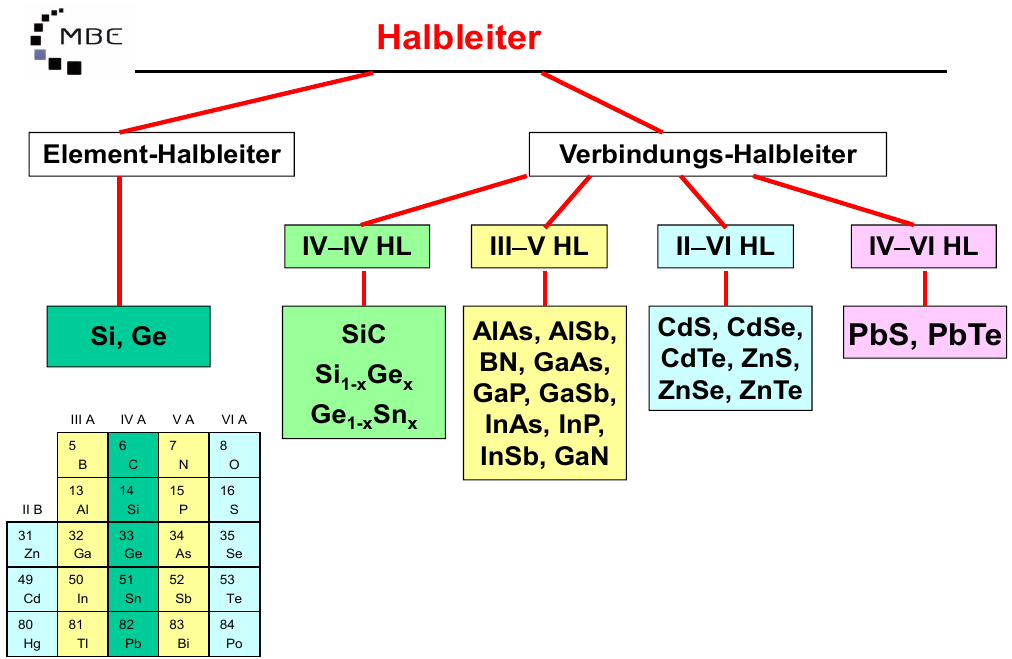
\includegraphics[width=0.8\textwidth]{Kapitel/Kap02/halbleiter.PNG}
		\caption{Halbleiter}
		\label{02_HL}
	\end{figure}
	\newpage
	
	
\subsection{Eigenschaften von Silizium}
	\subsubsection{Stellung im Periodensystem}
		Silizium befindet sich in der 4. Hauptgruppe und der 3. Periode im Periodensystem und hat die Ordnungszahl 14.
		\begin{figure}[h!]
			\centering
			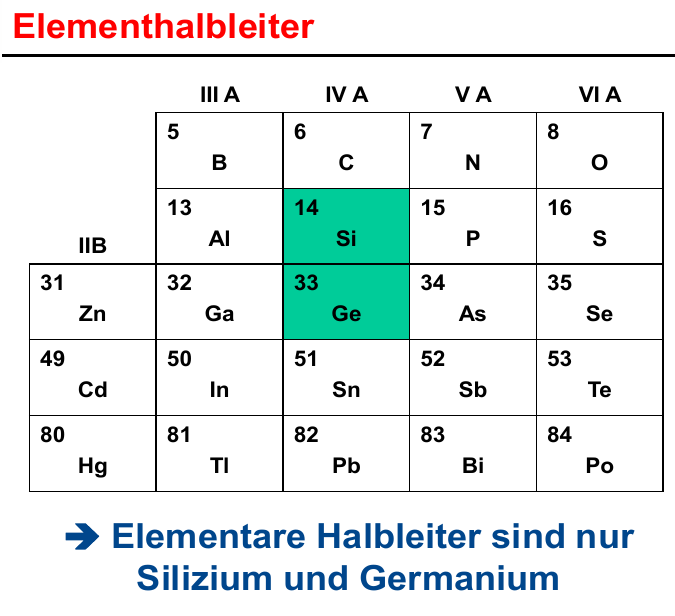
\includegraphics[width=0.5\textwidth]{Kapitel/Kap02/elementhalbleiter.PNG}
			\caption{Silizium im Periodensystem}
			\label{02_elementHL}
		\end{figure}
		
		
	\subsubsection{Valenzelektronen}
		Silizium ist ein indirekter Halbleiter. Damit ein ELektron aus dem Valenzband in das Leitungsband übergehen kann, muss ihm neben einer Energie auch noch ein Impuls zugeführt werden. Diese Art der Übergänge sind energetisch wenig wahrscheinlich.
		Die benötigte Energie ist hier die Energiedifferenz von Leitungsband zu Valenzband :
		\begin{equation*}
		E_g = E_{LB} - E_{VB}
		\end{equation*}
		
		Der benötigte Impuls beträgt:
		\begin{equation*}
			\Delta p = 2\pi h(k_{LB}-k_{VB})
		\end{equation*}
		
		Silizium hat eine Bandlücke von ca 1.1eV.
		
		\newpage
		\begin{figure}[ht]
			\centering
			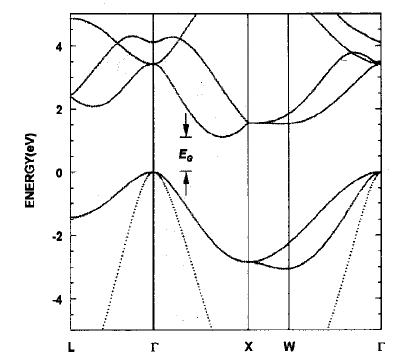
\includegraphics[width=0.5\textwidth]{Kapitel/Kap02/bandstruktur_SI.PNG}
			\caption{Bandstruktur von Silizium}
			\label{02_BS_SI}
		\end{figure}
		
	
	\subsubsection{Kristallstruktur}
		
		Kristallstruktur: Diamantstruktur
		Das Raumgitter besteht aus zwei kubisch-flächenzentrierten Gittern, die um 1/4 der Raumdiagonalen gegeneinander verschoben sind.
		Basis: identische Atome bei (0,0,0) und (1/4, 1/4, 1/4).
		Ein Si-Atom hat vier Außenelektronen, mit denen es Bindungen zu vier Nachbaratomen eingehen kann. Da (fast) alle Elektronen gebunden sind, ist die Leitfähigkeit (bei Raumtemperatur) sehr gering. (Das Valenzband ist (fast) vollständig besetzt, das Leitungsband hingegen (fast) vollständig leer.)
		
				
	\begin{figure}[h!]
		\centering
		\begin{minipage}[t]{0.35\linewidth}
			\centering
			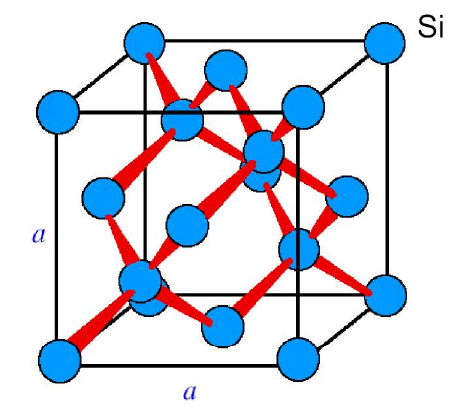
\includegraphics[width=\linewidth]{Kapitel/Kap02/Diamantstruktur_SI.PNG}
			\caption{Diamantstruktur von Silizium}
			\label{02_diamStruktur}
		\end{minipage}% <- sonst wird hier ein Leerzeichen eingefügt
		\hfill
		\begin{minipage}[t]{0.35\linewidth}
			\centering
			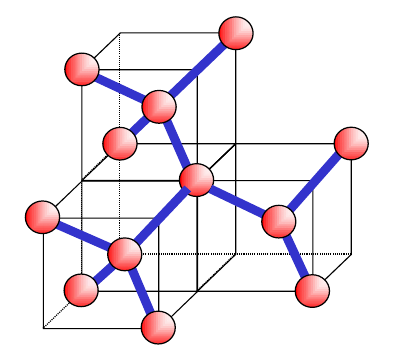
\includegraphics[width=\linewidth]{Kapitel/Kap02/raeumlichesModell_SI.PNG}
			\caption{räumliches Modell von Silizium}
			\label{02_raeumlModell}
		\end{minipage}
	\end{figure}

		
	\subsubsection{Miller'sche Indizes und Kristallorientierungen}
	
		In der heutigen Mikroelektronik wird überwiegend Si(001) genutzt.
		Die Oberfläche von Si(001) hat eine 4-fache Symmetrie, damit gibt es zwei freie Bindungen pro Oberflächenatom.
		Die Oberfläche von Si(111) hat dagegen eine 3-fache Symmetrie und damit nur eine freie Bindung pro Oberflächenatom.
		
		\begin{figure}[h]
			\centering
			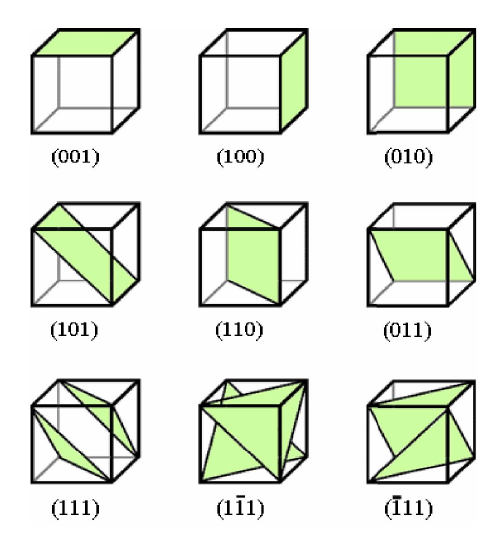
\includegraphics[width=0.22\textwidth]{Kapitel/Kap02/millerscheIndizes.PNG}
			\caption{Miller'sche Indizes}
			\label{02_millInd}
		\end{figure}
	
\subsection{Eigenleitung}
	T=0K: Alle möglichen Energiezustände im Valenzband sind von Elektronen besetzt. Das Leitungsband ist leer $\rightarrow$ es handelt sich um einen perfekten Isolator
	T>0K: Thermische Schwingungen können zur Bildung eines Elektron-Lochpaares führen. Die entstandenen freien Elektronen bedingen sich energetisch im Leitungsband. Die positiv geladenen Löcher verbleiben im Valenzband, sie sind dort ebenfalls beweglich.
	
	$Si \longrightarrow Si + e^- + h^+$ (e = electrons, h = holes)
	
	Im reinen Halbleiter finden Elektronenleitung \textbf{und} Löcherleitung statt. Die Anzahl von freien Elektronen und Löchern ist gleich: $\mathbf{n_i \cdot{p_i} = {n_i}^2}$
	
	\textbf{Generation:} Entstehung eines Elektron-Lochpaares
	\textbf{Rekombination:} Verschwinden eines Elektron-Lochpaares
	$\rightarrow$ hierbei fängt ein beliebiges Loch, unter Freigabe von Energie, ein beliebiges Elektron auf.
	
	Die Beweglichkeit von Elektronen ist immer sehr viel höher als die der Löcher.
	
\subsection{Dotierung}
	Die Eigenleitung von Halbleitern ist zu gering für eine technische Nutzung. Durch Dotierung (gezielte Verunreinigung mit Fremdatomen) wird die Leitfähigkeit erhöht. Die dotierten Materialien können überwiegend positive Ladungen (p-Typ) oder negative \textbf{freie} Ladungen (n-Typ) haben.
	Das \textbf{Massewirkungsgesetz} gilt aber auch für dotierte Halbleiter: $\mathbf{n \cdot{p} = {n_i}^2}$
	
	\subsubsection{Akzeptoren, Donatoren }
		\textbf{Donator:} ein Fremdatom der V-Hauptgruppe liefert ein zusätzliches Elektron
		Dotieren führt hier also zu einem Elektronenüberschuss $\rightarrow$ n-Leiter
		\begin{description}
			\item[$\bullet$] 5-wertige Stoffe sind z.B. Phosphor, Arsen, Antimon
			\item[$\bullet$] die abgegebenen Elektronen der Donatroren sind die (negativen) Ladungsträger
			\item[$\bullet$] es entstehen außerdem feste, positiv-geladene Ionen (tragen aber nicht zum Stromfluss bei)
			\item[$\bullet$] die Energieniveaus der Donatoren liegen dicht unterhalb des LB-Minimums in der Bandlücke ( $\rightarrow$ flache Störstelle)
		\end{description}
		
		\textbf{Akzeptor:} ein Fremdatom der III-Hauptgruppe kann ein Elektron aufnehmen
		Dotieren führt hier also zu einem Löcherüberschuss $\rightarrow$ p-Leiter
		\begin{description}
			\item[$\bullet$] 3-wertige Stoffe sind z.B. Bor, Gallium, ALuminium, Indium
			\item[$\bullet$] die entstehenden freien Löcher sind die (positiven) Ladungsträger
			\item[$\bullet$] es entstehen außerdem feste, negativ-geladene Ionen (tragen aber nicht zum Stromfluss bei)
			\item[$\bullet$] die Energieniveaus der Akzeptoren liegen dicht oberhalb des VB-Maximums in der Bandlücke ( $\rightarrow$ flache Störstelle)
		\end{description}
	
	\subsubsection{Konzentration, Lage im Bandgap usw.}
		
		
		\begin{figure}[h!]
			\centering
			\begin{minipage}[t]{0.45\linewidth}
				\centering
				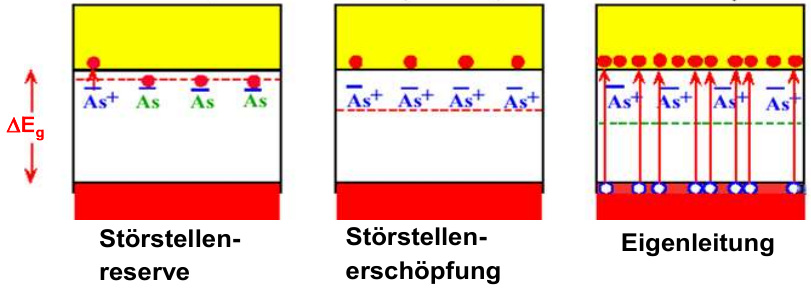
\includegraphics[width=1.2\textwidth]{Kapitel/Kap02/tempAbhSiAs.PNG}
				\caption{Dotieratomanregung am Beispiel von SiAs}
				\label{02_tempAbh}
			\end{minipage}% <- sonst wird hier ein Leerzeichen eingefügt
			\hfill
			\begin{minipage}[t]{0.45\linewidth}
				\centering
				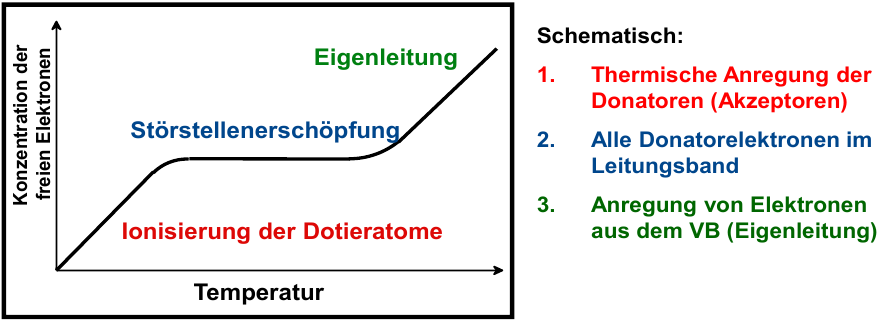
\includegraphics[width=1.2\textwidth]{Kapitel/Kap02/ladungstraegerkonzentration.PNG}
				\caption{T-Abhängigkeit der Ladungsträgerkonzentration (gilt auch für Akzeptoren)}
				\label{02_tempAbh2}
			\end{minipage}
		\end{figure}
		
		\begin{figure}[h!]
			\centering
			\begin{minipage}[t]{0.35\linewidth}
				\centering
				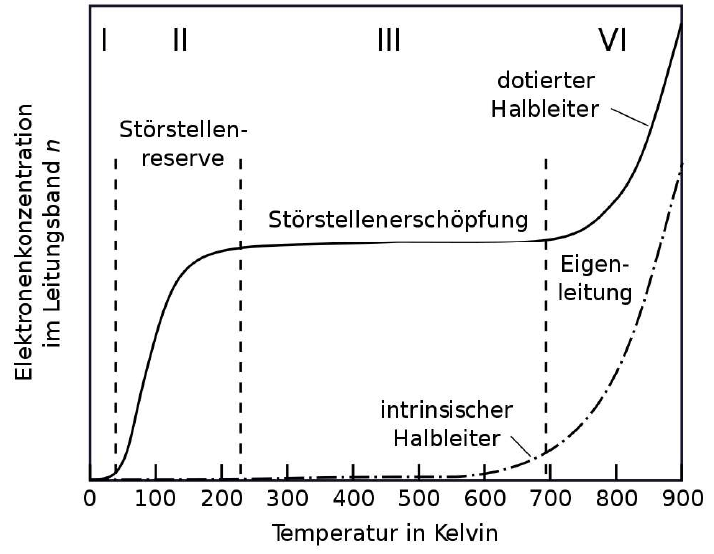
\includegraphics[width=\textwidth]{Kapitel/Kap02/tempAbh2.PNG}
				\caption{T-Abhängigkeit der Ladungsträgerkonzentration}
				\label{02_tempAbh3}
			\end{minipage}% <- sonst wird hier ein Leerzeichen eingefügt
			\hfill
			\begin{minipage}[t]{0.35\linewidth}
				\centering
				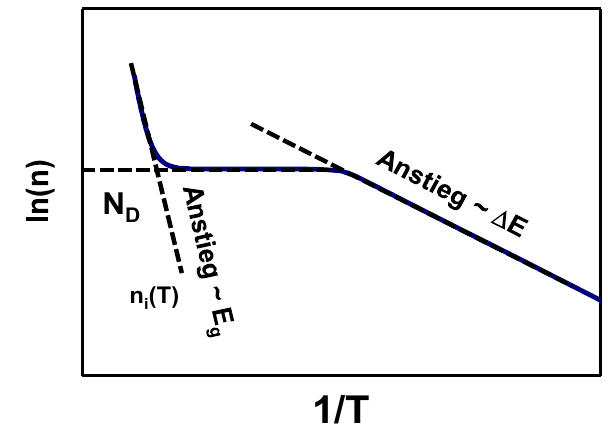
\includegraphics[width=\textwidth]{Kapitel/Kap02/tempAbh3.PNG}
				\caption{T-Abhängigkeit der Ladungsträgerkonzentration}
				\label{02_tempAbh4}
			\end{minipage}
		\end{figure}
		
		\newpage
		\textbf{Lage im Bandgap:}
		\begin{figure}[h!]
			\centering
			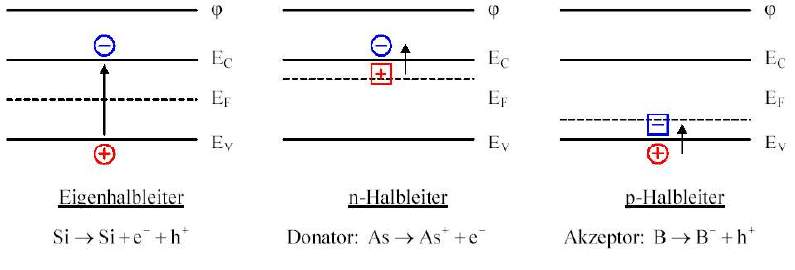
\includegraphics[width=0.9\textwidth]{Kapitel/Kap02/bandgapLage.PNG}
			\caption{Lage im Bandgap}
			\label{02_bandgap}
		\end{figure}
		
	\subsubsection{Dotantenaktivierung}
	DIe Anregung (Ionisation) wird als Aktivierung bezeichnet. Die Wahrscheinlichkeit für die Ionisation eines Donators ist von der Lage seines Energieniveaus $E_D$ abhängig. 
	Anzahl der Donatoren = neutrale + ionisierte ($N_D = {N_D}^0 + {N_D}^+$)
	\newpage
	
	\subsubsection{Dotiertechniken}
		\begin{figure}[h!]
			\centering
			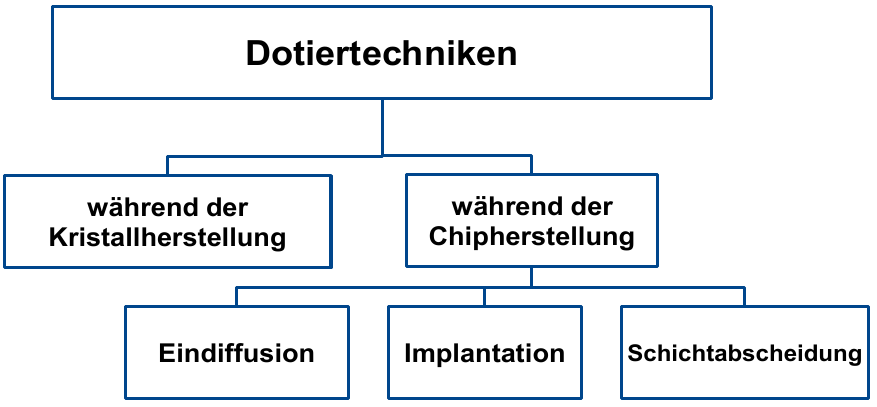
\includegraphics[width=0.7\textwidth]{Kapitel/Kap02/dotiertechniken.PNG}
			\label{02_dotiertechniken}
		\end{figure}
		
\subsection{Gewinnung von Reinstsilizium}

	\subsubsection{Reduktion im Niederschachtofen}
		Sand (Siliziumdioxid - $SiO_2$) wird bei ca 1450°C geschmolzen. Dabei wird Kohlenstoff zugegeben. Der Kohlenstoff verbindet sich mit dem Sauerstoff zu Kohlenmonoxid, was so aus der Schmelze entweicht. Die Reaktionsprodukte (Silizium und gasförmiges Kohlenmonoxid) lassen sich leicht trennen.
		\begin{figure}[h!]
			\centering
			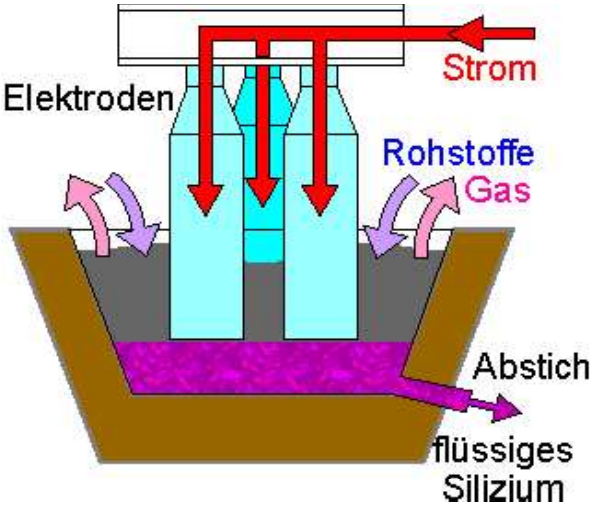
\includegraphics[width=0.4\textwidth]{Kapitel/Kap02/niederschachtofen.PNG}
			\caption{Niederschachtofen}
			\label{02_niederschachtofen}
		\end{figure}
		
	\subsubsection{Reinigung im Wirbelschichtreaktor}
		Das gewonnene Rohsilizium hat typischerweise immer noch Verunreinigungen von ca 2-4% , die entfernt werden müssen. Hierfür wird das Rohsilizium zu Trichlorsilan umgewandelt und anschließend fraktioniert destilliert. Um das Silizium umzuwandeln wird es zu einer Korngröße von ca 0.1mm gemahlen und dann in einem Wirbelschichtreaktor mit Chlorwasserstoff durchwirbelt. Unter Wärmeentwicklung entsteht als Reaktionsprodukt hauptsächlich Trichlorsilan.
		Trichlorsilan hat einen Siedepunkt von 30°C und kann deshalb in großen, mehrstufigen Destillationsanlagen von den Verunreinigungen befreit werden. Dieses gereinigte Trichlorsilan dient als Ausgangsstoff für die Herstellung von polykristalllinem Reinsilizium.
		
	\subsubsection{Polyabscheidung (Siemensprozess)}
		Trichlosilan und Wasserstoff werden in einen Abscheidungsreaktor geleitet. Dieser besteht aus einer Quarzglocke, in dem sich eine u-förmige Brücke aus dünnen Reinstsiliziumstäben (Dünnstab) befindet. Hier wird polykristallines Silizium abgeschieden. Durch den Dünnstab wird ein elektrischer Strom geleitet, der für die nötige Erwärmung auf die Reaktionstemperatur sorgt. (Je dicker der Stab wird, desto höher wird der Strom geregelt.) Das polykristalline Silizium hat nun eine Reinheit von 99,9999999% (9N).
\subsection{Einkristallines Silizium}
	Für die Chipherstellung wird einkristallines Silizium benötigt. Der Einkristall wird aus dem polykristallinen Silizium gezogen. Hierfür gibt es zwei Verfahren: Zonenziehen und Tiegelziehen im Schmelztiegel. Bei beiden Verfahren wird ein Impfkristall verwendet. Dies ist ein kleiner Einkristall mit einer genau definierten Ausrichtung des Kristallgitters. Die Kristallstruktur des erstarrenden Siliziums richtet sich genau an der des Impfkristalls aus $\Rightarrow$ Epitaxie
	
	\subsubsection{Zonenziehen und Tiegelziehen}
		\textcolor{red}{\textbf{Zonenziehen:}} (FZ-Verfahren)
			Silizium in Stabform wird mit einer Hochfrequenz-Induktionsspule direkt beheizt. Nach dem Anschmelzen wird der Schmelztropfen mit dem Impfkristall in Kontakt gebracht. Der sich drehende Stab wird durch die Spule abgesenkt und die Schmelzzone somit von unten nach oben gezogen.
			
			\textbf{Vorteile:}
				\begin{description}
					\item[$\bullet$] noch bestehenden Verunreinigungen werden in der Schmelze gelöst und so aus dem Stab herausgezogen
					\item[$\bullet$] Dotierungen, in Form von Prozessgasen, können gezielt vorgenommen und homogen in das Kristallgitter eingebaut werden
				\end{description}
			\textbf{Nachteile:}
			\begin{description}
				\item[$\bullet$] es lassen sich nur Stäbe von einem Durchmesser von 150mm sinnvoll ziehen
			\end{description}
				
			
		\textcolor{red}{\textbf{Tiegelziehen:}} (CZ-Verfahren)
		
		\begin{figure}[h!]
			\centering
			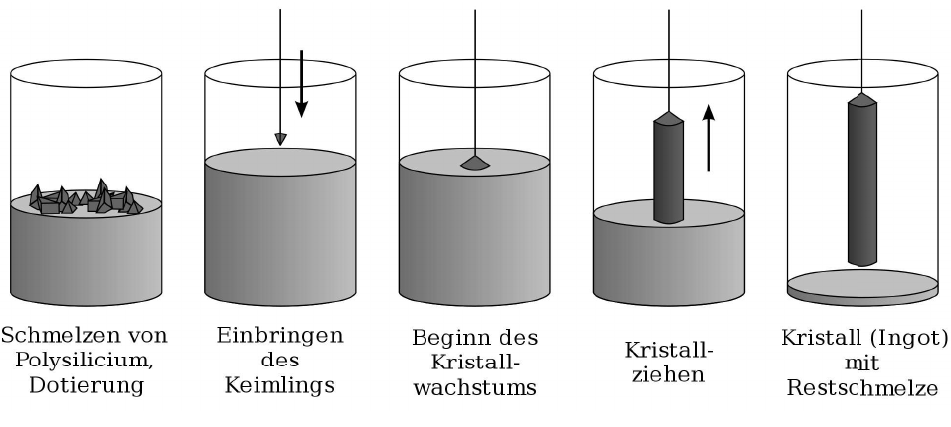
\includegraphics[width=\textwidth]{Kapitel/Kap02/tiegelziehen.PNG}
			\caption{Tiegelziehen}
			\label{02_tiegelziehen}
		\end{figure}
		
		\textbf{Vorteile:}
		\begin{description}
			\item[$\bullet$] ist vorallem für die Produktion von modernen großen Wafern geeignet (300mm und größer)
		\end{description}
		\textbf{Nachteile:}
		\begin{description}
			\item[$\bullet$] Dauer des Ziehprozesses: 1-3 Tage
			\item[$\bullet$] Inhomogenität bei der Vordotierung
			\item[$\bullet$] Verunreinigungen entstehen durch Kohlenstoff und Sauerstoff im Tiegel (die Verunreinigungen sind für viele Anwendungen aber gering genug)
		\end{description}
		
	\subsubsection{Zusammenfassung: Gewinnung von einkristallinem Silizium}
		\begin{description}
			\item[$\bullet$] \textbf{Gewinnung von Rohsilizium}
			\begin{description}
				\item[-] Reduktion im Niederschachtofen
				\item[-] Reinigung im Wirbelschichtreaktor $\rightarrow$ Umwandlung in Trichlorsilan
				\item[-] Polyabscheiung (Siemensprozess) $\rightarrow$ polykristallines Reinsilizium
			\end{description}
			\item[$\bullet$]Einkristallines Silizium
			\begin{description}
				\item[-] Zonenziehen oder Tiegelziehen
			\end{description}
			$\Rightarrow$ Einkristalline Si-Blöcke
		\end{description}
		
	\subsubsection{Wafermaße und -orientierungen}
		\begin{figure}[h!]
			\centering
			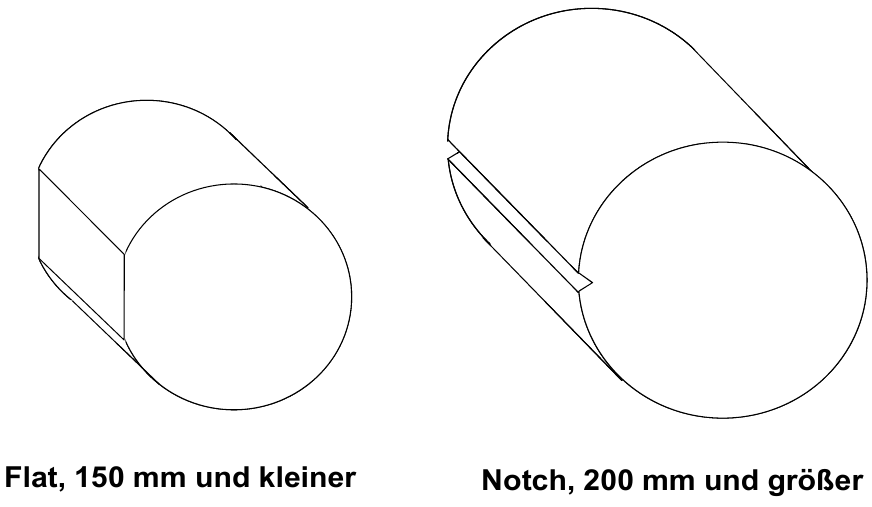
\includegraphics[width=0.4\textwidth]{Kapitel/Kap02/wafermasse.PNG}
			\caption{Flat oder Notch}
			\label{02_flat_notch}
		\end{figure}
		
		\begin{figure}[h!]
			\centering
			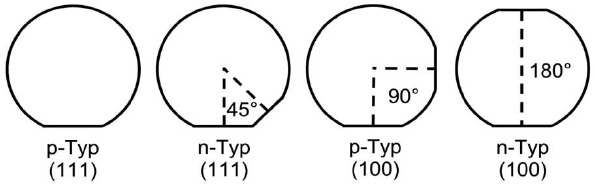
\includegraphics[width=0.6\textwidth]{Kapitel/Kap02/orientierungen.PNG}
			\caption{Waferherstellung: Flat}
			\label{02_flat}
		\end{figure}

	\todo{Fragen aus Own Clowd zuordnen}
	\todo{Gruppenübungs-Inhalte ergänze}
